% Created 2016-03-12 Sat 15:29
\documentclass[bigger]{beamer}
\usepackage[utf8]{inputenc}
\usepackage[T1]{fontenc}
\usepackage{fixltx2e}
\usepackage{graphicx}
\usepackage{longtable}
\usepackage{float}
\usepackage{wrapfig}
\usepackage{rotating}
\usepackage[normalem]{ulem}
\usepackage{amsmath}
\usepackage{textcomp}
\usepackage{marvosym}
\usepackage{wasysym}
\usepackage{amssymb}
\usepackage{hyperref}
\tolerance=1000
\usetheme{default}
\author{Weston Dransfield}
\date{\today}
\title{Completeness: 3Color}
\hypersetup{
  pdfkeywords={},
  pdfsubject={},
  pdfcreator={Emacs 24.5.1 (Org mode 8.2.10)}}
\begin{document}

\maketitle
\begin{frame}{Outline}
\tableofcontents
\end{frame}


\begin{frame}[label=sec-1]{Description}
\textbf{\textit{3COLOR}} = \{\(\langle G \rangle\) | the nodes of G can be colored with three colors such that no two adjacent nodes are the same color \}
\end{frame}

\begin{frame}[label=sec-2]{Example}
\begin{center}
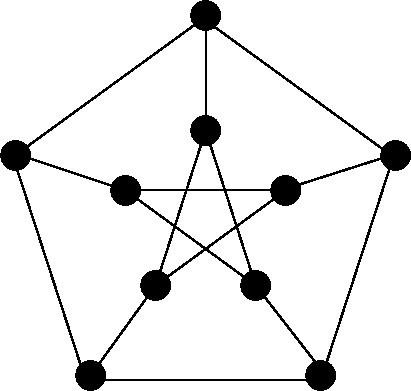
\includegraphics[width=7cm]{uncolored.jpg}
\end{center}
\end{frame}

\begin{frame}[label=sec-3]{Example}
\begin{center}
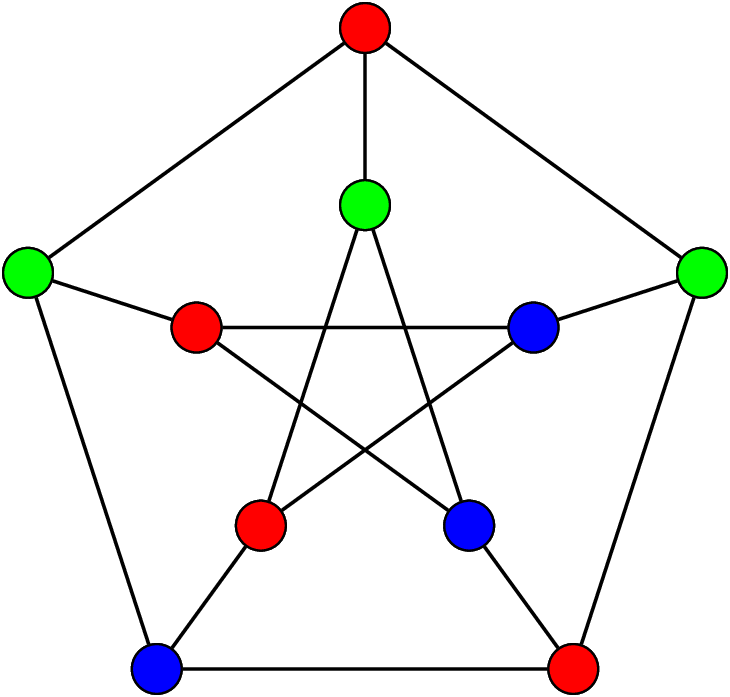
\includegraphics[width=7cm]{colored.png}
\end{center}
\end{frame}


\begin{frame}[label=sec-4]{The Problem}
Is a given graph \(G\) a member of the \textbf{\textit{3COLOR}}?

\begin{itemize}
\item<2-> This is tough to decide, but easy to verify!
\end{itemize}
\end{frame}

\begin{frame}[label=sec-5]{The Verifier}
\(V\) = "On input \(\langle G, c \rangle\),
\begin{enumerate}
\item<1-> Check that c includes 3 colors.
\item<2-> Color each node of G as specified by c.
\item<3-> For each node, check that each adjacent node is not the same color.
\item<4-> If all checks pass accept, otherwise reject."
\end{enumerate}

\begin{itemize}
\item<5->Step 3 has largest time complexity of \(O(n^2)\). 3COLOR is in NP because it can be verified in polynomial time.
\end{itemize}
\end{frame}
% Emacs 24.5.1 (Org mode 8.2.10)
\end{document}
